%%      VTU Intern Report Template using LaTeX  2020
%%      
%%      Copyright 2020 vivekadi <vivek.adishesha@gmail.com>,
%%		keshavbharadwaj <keshavbharadwaj@gmail.com>, 
%%		anirudhMkndn <anirudhmanikandan98@gmail.com>,
%%		sharathnpayyadi <sharathnp1998@gmail.com>,
%%		chiranjitpatel <chiranjitpatel08@gmail.com>
%%		vivekurankar <vivekurankar@gmail.com>,
%%      sadi3491 <souravadi1998@gmail.com>,
%%		suhas <suhasraikar46@gmail.com>,
%%		
%%      This program is FREE SOFTWARE; you can redistribute it and/or modify
%%      it under the terms of the GNU General Public License as published by
%%      the Free Software Foundation; either version 2 of the License, or
%%      (at your option) any later version.
%%      
%%      This program is distributed in the hope that it will be useful,
%%      but WITHOUT ANY WARRANTY; without even the implied warranty of
%%      MERCHANTABILITY or FITNESS FOR A PARTICULAR PURPOSE. See %%            the%\AddToShipoutPicture{\setlength\fboxsep{8pt}\put(25,25){\framebox(7.65in,11.08in)[lb]{}}}
\abstractintoc
\thispagestyle{plain}
\renewcommand{\abstractname}{Abstract}
\renewcommand{\abstractnamefont}{\Large\textbf}
\renewcommand{\abstracttextfont}{\normalsize}
\begin{abstract}
\OnehalfSpacing

{\LaTeX} eases our pressure in writing thesis \& reports because of its powerful features such as automatic hyphenation, table of contents, figures \& tables,  powerful bibliography tool, citations,Automatic Numbering of Chapter, sections, figures \& tables, its beautiful fonts, professional output...

Writing too much of code for gives bad impression on {\LaTeX}. But now we have numerous gui tools like gedit-latex-plugin, {\TeX}maker, Lyx \& emacs, which are very much user friendly. 

This VTU-project-report-template is written using popular document class, ``Memoir". In the coming chapters, we hav given small help manual required for writing report \& at the end about template

\end{abstract}

%%      GNU General Public License for more details.
%%      
%%      You should have received a copy of the GNU General Public License
%%      along with this program; if not, write to the Free Software
%%      Foundation, Inc., 51 Franklin Street, Fifth Floor, Boston,
%%      MA 02110-1301, USA.


%%%%%%%%%%%%%%%%%%%%%%%%%%%%%%%%%%%%%%%%%%%%%%%%%%%%%%%%%%%%%%%%%%%%%%%%%
%
\documentclass[12pt,a4paper,oneside]{memoir}
\usepackage{graphicx}
\usepackage[english]{babel}
\usepackage[a4paper,right=1in]{geometry}
\usepackage{hyperref}
\usepackage{listings}
\usepackage{pdfpages}
\usepackage{float}
\usepackage{xcolor}
\usepackage{afterpage}
%\usepackage{background}
\usepackage{amsmath}
\usepackage{subcaption}
\usepackage{rotating}
\usepackage{tabularx}
\usepackage{caption}
\usepackage{mwe}
\usepackage{lipsum}
\usepackage{multirow}
\usepackage{wrapfig}
\usepackage{moresize}



\renewcommand{\afterchapternum}{\par\bigskip}
\setlength{\beforechapskip}{-2\baselineskip}
%To reduce%the Chapter vertical height.


%document starts here
\begin{document}
	\newlength{\toptafiddle} 
	\newlength{\bottafiddle}
	%\definecolor{rnspurple}{rgb}{0.25,0.04,0.43}
\usetikzlibrary{calc}
\SetBgScale{1}
\SetBgAngle{0}
\SetBgColor{white}
\SetBgOpacity{1}
\SetBgContents							% To apply page borders.
{
	\begin{tikzpicture}[overlay,remember picture]
	\draw [line width=1.5pt]
	($ (current page.north west) + (1.0cm,-1.0cm) $)
	rectangle
	($ (current page.south east) + (-1.0cm,1.0cm) $);
	\end{tikzpicture}
}

\begin{titlingpage}
	%\clearpage
	\thispagestyle{empty}\centering
	\pagecolor{rnspurple}\afterpage{\nopagecolor}
	
\setlength{\toptafiddle}{1in}
\setlength{\bottafiddle}{1in}
\vspace*{-0.75in}
\enlargethispage{\toptafiddle}
\large 
\textbf{\color{white}VISVESVARAYA TECHNOLOGICAL UNIVERSITY\\
	Jnana Sangama, Belagavi - 590 018}\\
\vspace{0.2cm}
\begin{figure}[h]
	\centering
	\includegraphics[height=3cm]{images/vtu.png}
\end{figure}
\small{\textbf{\color{white}PROJECT REPORT ON}}\\

\LARGE{\textbf{\color{white}Title of the Project}}
\vspace{0.5cm}

\large \textit{\color{white}Thesis submitted in partial fulfillment for the Award of Degree of }{\textbf{\color{white}Bachelor of Engineering}}\\
\color{white} in \\\textbf{\color{white}Electronics and Communication Engineering}
\vspace{0.5cm}\\
{\textbf{\color{white}Submitted by\\}}


\begin{tabular}{lll}
	
\color{white}	Name1 & \hspace{5cm} & \color{white}1RN16EC\\
\color{white}	Name2 &   & \color{white}1RN16EC\\
\color{white}	Name3 &   & \color{white}1RN16EC\\
\color{white}	Name4 &   & \color{white}1RN16EC\\
	
\end{tabular}
\vspace{0.5cm}\\
\textit{\color{white}Under the Guidance of}


\Large{\textbf{\color{white}Name}}\\
\textit{\color{white}Designation}\\

\begin{figure}[h]
	\centering
	
\includegraphics[height=2.7cm]{images/rns1.jpg}
\end{figure}


\begin{center}
	\scriptsize\textbf{\color{white}DEPARTMENT OF ELECTRONICS AND COMMUNICATION ENGINEERING}\\
	\small\textbf{\color{white}(Accredited by NBA for the Academic years 2018-19, 2019-20 and 2020-21)}	
\end{center}
\begin{center}
	\vspace{0.1cm}
	\large\textbf{\color{white}RNS INSTITUTE OF TECHNOLOGY}\\
	\small\textbf{\color{white}(AICTE Approved, VTU Affiliated and NAAC `A' Accredited)\\
		(UG Programs - CSE, ECE, ISE, EIE and EEE have been Accredited by NBA for the Academic years 2018-19, 2019-20 and 2020-2021)\\
		Channasandra, Dr.Vishnuvardhan Road, Bengaluru-560098\\
		2019 - 20}
\end{center}
\end{titlingpage}

	%\AddToShipoutPicture{\setlength\fboxsep{8pt}\put(25,25){\framebox(7.65in,11.08in)[lb]{}}}


\begin{titlingpage}
%\clearpage
\thispagestyle{empty}\centering

\begin{figure}[H]
	\centering
	\includegraphics[width=0.7\linewidth]{"images/logo_no_bg copy"}
\end{figure}



%\Huge{\textbf{\color{red}Title of the Project}}
\vspace{1.2cm}
\scalebox{2}{\fontsize{22pt}{0pt}\selectfont \textbf{\color{red}Q - CERGEN}}
\vspace{1.2cm}

\Large \textit{\textbf{E - Certificate Generator User Manual}}\\
\Large \textit{\textbf{for}}\\
\vspace{0.4cm}
\Large \textit{\textbf{Quick - Certificate Generator Software}}\\
\Large \textit{\textbf{Version 3.1}}

\vspace{2.5cm}
\normalsize\textit{\textbf{Towards swift, perfect \& authentic certifications}}




\end{titlingpage}
%include titlepage,i.e, title.tex file
	%Page layout according to VTU specification
	%Right=1.25in,left=1in, Top & Bottom 0.75in in each
	
	\setlength{\oddsidemargin}{0.25in}%left side margin{1in by default+0.25in}
	
	%header specification
	\setlength{\headheight}{\onelineskip}
	\setlength{\headsep}{4pt}
	\setlength{\topmargin}{-0.25in}
	
	%footer specification
	\setlength{\footskip}{0.7cm}
	\setlength{\footnotesep}{0.7cm}
	
	%A4 paper height = 11.69in
	%thus 11.69in-9.67in-1in(top+header) is approx 0.75in left for bottom
	\setlength{\textheight}{9.60in}
	\brokenpenalty=10000
	\OnehalfSpacing
	
	%%\AddToShipoutPicture{\setlength\fboxsep{8pt}\put(25,25){\framebox(7.65in,11.08in)[lb]{}}}
\setlength{\toptafiddle}{1in}
\setlength{\bottafiddle}{1in}
\vspace*{-0.5in}
\enlargethispage{\bottafiddle}
\thispagestyle{empty}


\begin{center}
	\large\textbf{RNS INSTITUTE OF TECHNOLOGY}\\
	\small\textbf{(AICTE Approved, VTU Affiliated and NAAC `A' Accredited)\\
		(UG Programs - CSE, ECE, ISE, EIE and EEE have been Accredited by NBA for the Academic years 2018-19, 2019-20 and 2020-2021)\\
		Channasandra, Dr.Vishnuvardhan Road, Bengaluru-560098}\\
\end{center}
\begin{center}
	\footnotesize\textbf{DEPARTMENT OF ELECTRONICS AND COMMUNICATION ENGINEERING}
	\small\textbf{(Accredited by NBA for the Academic years 2018-19, 2019-20 and 2020-21)}	
\end{center}

\begin{center}
\begin{figure}[h]
\centering

\includegraphics[height=2.7cm]{images/rns1.jpg}
\end{figure}
\Large{\textbf{CERTIFICATE}}
\end{center}

Certified that the Thesis work entitled \textbf{``Title of the Project Report''} is carried out by \textbf{Student-1(USN), Student-2(USN), Student-3(USN), and Student-4(USN)} in partial fulfillment for the award of degree of Bachelor of Engineering in \textbf{\color{blue}Electronics and Communication Engineering} of Visvesvaraya Technological University, Belagavi, during the year 2019-2020. It is certified that all corrections / suggestions indicated during internal assessment have been incorporated in the report. The project report has been approved as it satisfies the academic requirements in aspect of the project work prescribed for the award of degree of \textbf{\color{blue}Bachelor of Engineering}.

\vspace{1.2cm}
\begin{minipage}[t]{0.3\textwidth}%
	\small{\color{gray!35}................................}\\
	{\centering{\color{red}Name of the Guide}}\\
	\centering{Designation}\\
\end{minipage}\hspace{0.06cm}
\begin{minipage}[t]{0.3\textwidth}%
	\small{\color{gray!35}................................}\\
	{\centering{\color{red}Dr. Vipula Singh}}\\
	\centering{Head of the Department}\\
\end{minipage}
\begin{minipage}[t]{0.3\textwidth}%
	\small{\color{gray!35}................................}\\
	{\centering{\color{red}Dr. M K Venkatesha}}\\
	\centering{Principal}\\
\end{minipage}

\vspace{0.1cm}
\begin{center}
	\textbf{{\color{blue}External Viva}}
\end{center}

\vspace{0.1cm}
\begin{minipage}[t]{0.62\textwidth}%
	\textbf{Name of the examiners}\\\\
	1 \small{\color{gray!35}..........................................}\\
	\\
	2 \small{\color{gray!35}..........................................}\\
\end{minipage}\hspace{0.07cm}
\begin{minipage}[t]{0.62\textwidth}%
	\textbf{Signature with date}\\\\
	\small{\color{gray!35}...........................................}\\
	\\
	\small{\color{gray!35}...........................................}\\
\end{minipage}

	%
%\AddToShipoutPicture{\setlength\fboxsep{20pt}\put(25,25){\framebox(7.65in,11.08in)[lb]{}}}
\setlength{\toptafiddle}{1in}
\setlength{\bottafiddle}{1in}
\vspace*{-0.5in}
\enlargethispage{\bottafiddle}
\thispagestyle{empty}


\begin{center}
	\large\textbf{RNS INSTITUTE OF TECHNOLOGY}\\
	\small\textbf{(AICTE Approved, VTU Affiliated and NAAC `A' Accredited)\\
		(UG Programs - CSE, ECE, ISE, EIE and EEE have been Accredited by NBA for the Academic years 2018-19, 2019-20 and 2020-2021)\\
		Channasandra, Dr.Vishnuvardhan Road, Bengaluru-560098}\\
		\vspace{0.1cm}
\end{center}
\begin{center}
		\footnotesize\textbf{DEPARTMENT OF ELECTRONICS AND COMMUNICATION ENGINEERING}
		\small\textbf{(Accredited by NBA for the Academic years 2018-19, 2019-20 and 2020-21)}	
\end{center}

\begin{center}
\begin{figure}[h]
\centering

\includegraphics[height=2.7cm]{images/rns1.jpg}
\end{figure}
\Large{\textbf{\color{red}{DECLARATION}}}
\end{center}

We here by declare that the entire work emobodied in this project report titled, \textbf{\color{red}``Title of Project"} submitted to \textbf{\color{red}Visvesvaraya Technological University}, Belagavi, is carried out at the department of             \textbf{\color{blue}Electronics and Communication Engineering, RNS Institue of Technology, Bengaluru} under the guidance of \textbf{\color{blue}Name of the Guide}, Designation. This report has not been submitted for the award of any Diploma or Degree of this or any other University.


\vspace{1.5cm}
\begin{minipage}[t]{0.45\textwidth}%

\textbf{\hspace{1.5cm}Name\\\\
1. \\\\
2. \\\\
3. \\\\
4. \\\\
}
\end{minipage}\hspace{0.4cm}
\begin{minipage}[t]{0.3\textwidth}%

\textbf{\hspace{0.7cm}USN\\\\
1RN16EC \\\\
1RN16EC \\\\
1RN16EC \\\\
1RN16EC \\\\
}
\end{minipage}
\begin{minipage}[t]{0.3\textwidth}%

\textbf{\hspace{0.2cm}Signature}\\\\
\small{\color{gray!35}.........................}\\\\
\small{\color{gray!35}.........................}\\\\
\small{\color{gray!35}.........................}\\\\
\small{\color{gray!35}.........................}\\\\
\end{minipage}

	%\thispagestyle{empty}
	
\begin{figure}[h]
	\centering
	\includegraphics[height=24cm, width=15cm]{images/certificate.png}
\end{figure}
	
	\pagenumbering{roman}
	\pagestyle{plain}
	%%\AddToShipoutPicture{\setlength\fboxsep{8pt}\put(25,25){\framebox(7.65in,11.08in)[lb]{}}}
\abstractintoc
\thispagestyle{plain}
\renewcommand{\abstractname}{Abstract}
\renewcommand{\abstractnamefont}{\Large\textbf}
\renewcommand{\abstracttextfont}{\normalsize}
\begin{abstract}
\OnehalfSpacing

{\LaTeX} eases our pressure in writing thesis \& reports because of its powerful features such as automatic hyphenation, table of contents, figures \& tables,  powerful bibliography tool, citations,Automatic Numbering of Chapter, sections, figures \& tables, its beautiful fonts, professional output...

Writing too much of code for gives bad impression on {\LaTeX}. But now we have numerous gui tools like gedit-latex-plugin, {\TeX}maker, Lyx \& emacs, which are very much user friendly. 

This VTU-project-report-template is written using popular document class, ``Memoir". In the coming chapters, we hav given small help manual required for writing report \& at the end about template

\end{abstract}

	

\begin{titlingpage}
	
\vspace{2cm}

\centering
{
	\Large{
		\textbf{Q - CERGEN}\\
		\textbf{E - Certificate Generator}\\
		\textbf{\textit{Version 3.1}}}
	\vspace{2cm}
	
	\Large\textbf{Q - CERGEN}\\
	\vspace{0.5cm}
	\large\textbf{\textit{Keshav V Bharadwaj, Raghava R P, Shankar Anabalgan, Sourav P Adi, Vivek B A}}
	\vspace{2.5cm}
}


The creator of the certificates agrees to the license agreement file. The generator of the certificates authorizes the creation of each certificate and is solely responsible for the authenticity of the information. The developers of the software aren't responsible for the certificates generated by the issuing authority who has complied with the above conditions.

\vspace{2cm}

No part of this manual may be reproduced or distributed in any form or by any means, electronic, mechanical, photocopying, recording, or otherwise or stored in a database or retrieval system without the prior written permission of the developer.

\vspace{0.5cm}

\begin{flushleft}
	\large\textit{\textbf{Contact Us:}}\\
	\textit{\textbf{Email:} keshavbharadwaj98@gmail.com / vivek.adishesha@gmail.com}\\
	%\textit{\textbf{Phone:} +91 944-904-0813 / +91 948-365-8134}
\end{flushleft}
	
	
	
	
\end{titlingpage}



	

\renewcommand{\abstractname}{Preface}
\renewcommand{\abstractnamefont}{\Huge\textbf}
\renewcommand{\abstracttextfont}{\normalsize}
\begin{abstract}
	
Traditional certificates with perforated edges have been the essence of earning an award. They play a role in acknowledging the person of the achievements earned. They serve an authentic message from the issuer about accomplishment to anyone who lay eyes on it.\\

Traditional certificates come with an incurred burden when the number of people getting certified grows. The generation of handmade or paper-based certificates takes from a week to a month. The details are can be erroneous as they are written by hand, re-issuing of such increase costs and time. Authentication and maintenance of the database for numerous certificates becomes a frantic work The cost and usage of paper also make traditional certificates not to be preferred in the current $ 21^{st}$ century.\\

Digitized E-Certificates can be generated within minutes and sent to the receiver via an e-mail or by uploading it on the cloud. A large number of certificates can be generated with minimal errors, also the errors can be rectified instantaneously. No postal costs and no downtime for hand written content. The e-certificates can be employed with security features involving advanced cryptographic techniques such as steganography and secure hash functions.\\

The Q-CERGEN software is aimed to facilitate the generation of such authentic and foolproof e-certificates. User-friendly interface with secured accounts and can generate a minimum of 3 certificates per second.


\vspace{0.5cm}
\begin{flushright}\textbf{Keshav V Bharadwaj}\end{flushright}
\begin{flushright}\textbf{Shankar Anbalagan}\end{flushright}
\begin{flushright}\textbf{Sourav P Adi}\end{flushright}
\begin{flushright}\textbf{Vivek B A}\end{flushright}

\vfill
\end{abstract}




	

\renewcommand{\abstractname}{Acknowledgement}
\renewcommand{\abstractnamefont}{\Large\textbf}
\renewcommand{\abstracttextfont}{\normalsize}
\begin{abstract}
	\OnehalfSpacing
	
	
	We are indebted to a number of individuals who have contributed and assisted in the development of the software. Their contributions are the reflection of the performance from this software in its \textbf{Version 3.1}.\\
	
	We express our gratitude to \textbf{Wg Cdr S N Shridhara (Retd)} for his guidance and advice in the development of the software for engineering institutions.\\
	
	We wish to extend our appreciation to \textbf{Chiranjit Patel}, \textbf{Raghava R P}, \textbf{Sharath Payyadi}, \textbf{Sumanth M Bhat}, and \textbf{Vivek Urankar} for their assistance in data creation, analysis, and event managemnet for the generation of certificates.\\
	
	We express our profound gratitude to \textbf{Venkata Reddy} for his invaluable support in gaining copyrights for the Q - CERGEN software.\\
	
	We extend our earnest gratitude and respect to our parents and all our friends who have directly or indirectly supported us.
	
	
	\vspace{2cm}
	\begin{flushright}\textbf{Keshav V Bharadwaj}\end{flushright}
	\begin{flushright}\textbf{Shankar Anbalagan}\end{flushright}
	\begin{flushright}\textbf{Sourav P Adi}\end{flushright}
	\begin{flushright}\textbf{Vivek B A}\end{flushright}
	
	\vfill
\end{abstract}




	%%\AddToShipoutPicture{\setlength\fboxsep{8pt}\put(25,25){\framebox(7.65in,11.08in)[lb]{}}}
\abstractintoc
\thispagestyle{plain}
\renewcommand{\abstractname}{Abstract}
\renewcommand{\abstractnamefont}{\Large\textbf}
\renewcommand{\abstracttextfont}{\normalsize}
\begin{abstract}
\OnehalfSpacing

{\LaTeX} eases our pressure in writing thesis \& reports because of its powerful features such as automatic hyphenation, table of contents, figures \& tables,  powerful bibliography tool, citations,Automatic Numbering of Chapter, sections, figures \& tables, its beautiful fonts, professional output...

Writing too much of code for gives bad impression on {\LaTeX}. But now we have numerous gui tools like gedit-latex-plugin, {\TeX}maker, Lyx \& emacs, which are very much user friendly. 

This VTU-project-report-template is written using popular document class, ``Memoir". In the coming chapters, we hav given small help manual required for writing report \& at the end about template

\end{abstract}

	
	
	\setcounter{secnumdepth}{3}%sections numbering upto 3 level
	\renewcommand{\contentsname}{Table of Contents}
	\tableofcontents
	%\newpage
	%\listoffigures
	%\newpage
	%\listoftables 
	
	%\chapter*{Acronyms}
\addcontentsline{toc}{chapter}{Acronyms}

\begin{description}
	\item[PCB] : Printed Circuit Board
	
\end{description}


% For adding addition items copy paste the above lines of \item[PCB]
	
	
	\pagestyle{myheadings}
	\makeheadrule{myheadings}{\textwidth}{0.4pt}
	\makefootrule{myheadings}{\textwidth}{0.4pt}{\footruleskip}
	\makeoddhead{myheadings}{\small{Q - CERGEN}}{}{\small{$rho - vector $}}
	\makeoddfoot{myheadings}{\small{$rho - vector $}}{}{\small{\thepage}}
	
	\pagenumbering{arabic}
	
	
	\index{key}
	
	\chapter{Login}

Navigation in the login screen and creation of new accounts. Resetting the password of exixting accounts are done through this page. Theoutlook is depicted below, fields the user to enter are Email-ID, Password and Admin Key as per requirements.  

\begin{figure}[H]
	\centering
	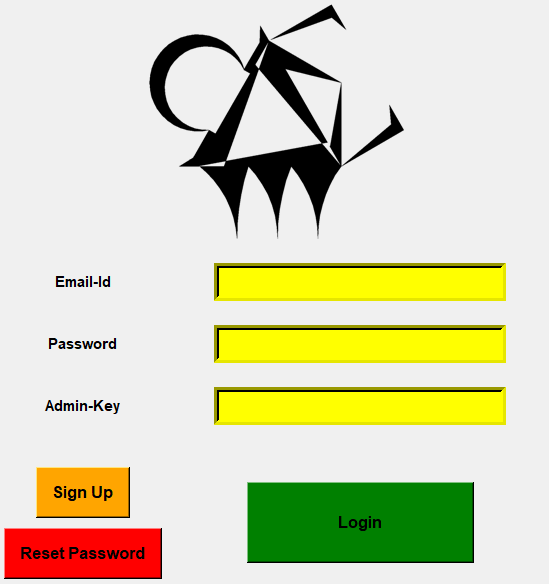
\includegraphics[width=0.6\linewidth]{images/login_page/login_1}
	\label{fig:login1}
\end{figure}

\section{Create New Account}

\begin{itemize}
	\item To create a new account, enter a working Email-ID, and a password of your choice.
	\item Preferably the password must have 8 characters with a special character
	\item The Admin Key is a must, please contact the Admin or Developer of the software in Contact Us
	\item All 3 fields must be entered, now clicking Sign-Up will create the account
	\item Please check verification email to the mail id provided, you can use the new account
\end{itemize}
\begin{figure}[H]
	\centering
	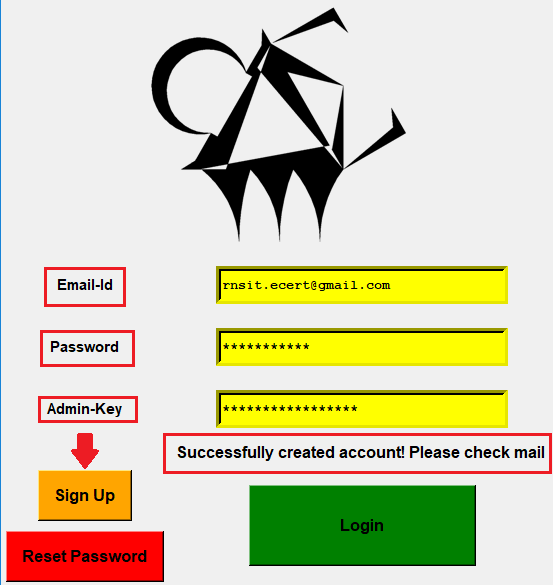
\includegraphics[width=0.6\linewidth]{images/login_page/login_4}
	\label{fig:login4}
\end{figure}

\begin{figure}[H]
	\centering
	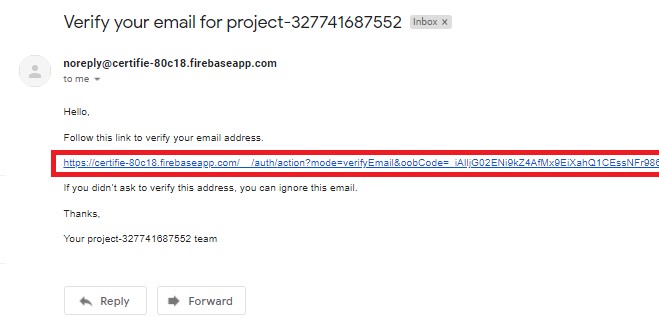
\includegraphics[width=0.9\linewidth]{images/login_page/login_6}
	\label{fig:login6}
\end{figure}

\begin{figure}[H]
	\centering
	
\includegraphics[width=0.95\linewidth]{images/login_page/login_5}
	\label{fig:login5}
\end{figure}

\section{Login with existing Account}

\begin{figure}[H]
	\centering
	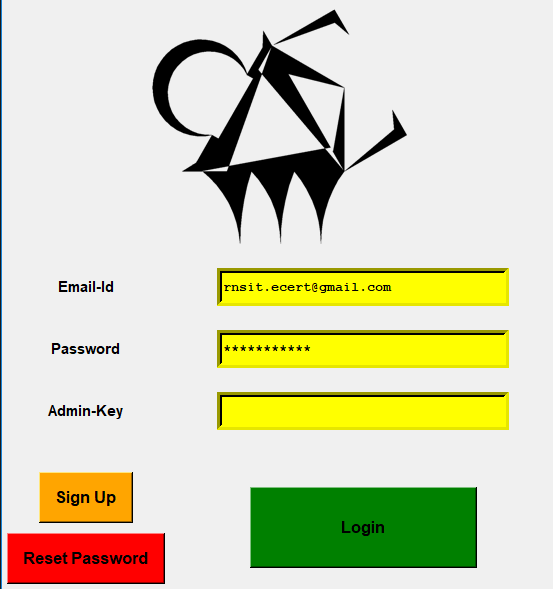
\includegraphics[width=0.45\linewidth]{images/login_page/login_2}
	\label{fig:login2}
\end{figure}


\begin{figure}[H]
	\centering
	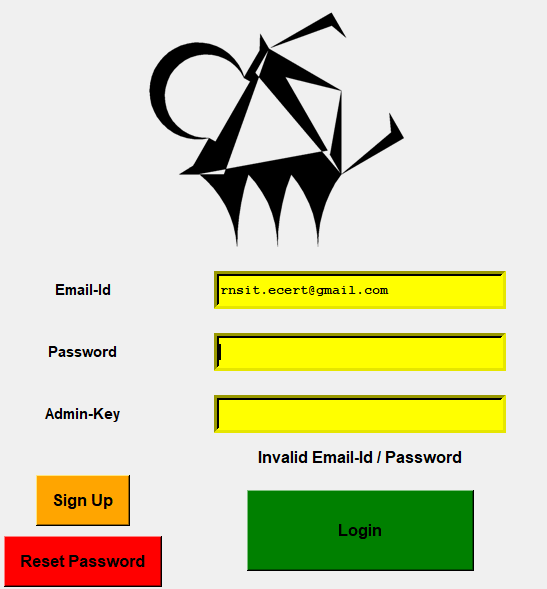
\includegraphics[width=0.45\linewidth]{images/login_page/login_3}
	\label{fig:login3}
\end{figure}

\section{Reset Password}


\begin{figure}[H]
	\centering
	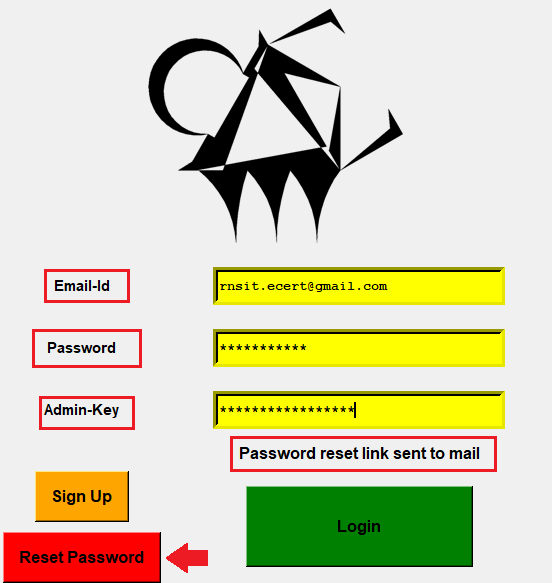
\includegraphics[width=0.6\linewidth]{images/login_page/login_7}
	\label{fig:login7}
\end{figure}






	%\chapter*{Organisation of Report}
\addcontentsline{toc}{chapter}{Organisation of Report}

	THREE to FOUR lines of description of each chapter included
\begin{description}
	\item[Chapter 1 :] 
	\item[Chapter 2 :] 
	\item[Chapter 3 :] 
	\item[Chapter 4 :]
	\item[Chapter 5 :]
	\item[Chapter 6 :]
\end{description}

	\chapter{Generation with QR / without QR Code}

The mainframe of the generator is as shown below. It is provided with three fuctionalities, generation, database, decoding the later two will be discussed in the outcoming chapter. Here the procedure to generate e-certificates with QR Code and without QR Code are discussed.


\begin{figure}[H]
	\centering
	\includegraphics[width=0.85\linewidth]{"images/generation_qr_nqr/Screenshot (28)"}
	\label{fig:screenshot-28}
\end{figure}

\newpage
\paragraph{1. Selection of Certificate template}
A certificate template must be created in JPG or PNG format in the host computer. Clicking on the Generation button pops up a window to select the certificate template image. This template can be created in Corel Draw or Adobe Photoshop.

\begin{figure}[H]
	\centering
	\includegraphics[width=0.85\linewidth]{"images/generation_qr_nqr/Screenshot (29)"}
	\label{fig:screenshot-29}
\end{figure}


\begin{figure}[H]
	\centering
	\includegraphics[width=0.85\linewidth]{"images/generation_qr_nqr/Screenshot (30)"}
	\label{fig:screenshot-30}
\end{figure}

\newpage
\paragraph{2. Steganography}

\begin{itemize}
	\item You can choose to embed a alpha-numeric code as securit code. This will be embedded into the certificate by steganography. If you have the password then you can enter your code number.
	\item If you don't have access to the password we are sorry this feature is not enabled for you!!, go back \& select `No' to continue with generation. With `No' a Default code will be inserted in steganography.
	\item Please contact Admin / Developer for the password incase the feature is necessary
\end{itemize}

\begin{figure}[H]
	\centering
	\includegraphics[width=0.5\linewidth]{"images/generation_qr_nqr/Screenshot (31)"}
	\label{fig:screenshot-31}
\end{figure}

\begin{figure}[H]
	\centering
	\includegraphics[width=0.65\linewidth]{"images/generation_qr_nqr/Screenshot (33)"}
	\label{fig:screenshot-33}
\end{figure}

\begin{figure}[H]
	\centering
	\includegraphics[width=0.5\linewidth]{"images/generation_qr_nqr/Screenshot (34)"}
	\label{fig:screenshot-34}
\end{figure}

\newpage
\paragraph{3. CSV / Data File selection}

\begin{itemize}
	\item Click `Yes' for CSV file
	\item Create the data in row and cloumns and save it in `.csv' format
	\item \textbf{Make sure there are no columns named as `img' or `serial'}
\end{itemize}

\begin{figure}[H]
	\centering
	\includegraphics[width=0.85\linewidth]{"images/generation_qr_nqr/Screenshot (37)"}
	\caption{}
	\label{fig:screenshot-37}
\end{figure}

\begin{figure}[H]
	\centering
	\includegraphics[width=0.9\linewidth]{"images/generation_qr_nqr/Screenshot (38)"}
	\caption{}
	\label{fig:screenshot-38}
\end{figure}

\newpage
\paragraph{4. Choosing QR code / No QR Code}
\begin{itemize}
	\item You can select whether QR Authentication with SHA-3 Hashing must be provided or not for the certificates
	\item If `No', then you'll be taken to select the required columns that come up on the certificate
	\item If 'Yes' you'll have to wait for few moments to create the QR codes and Authentication links for verification. After the links generated you'll have to select the columns required for the certificate
	\item \textit{Adiced to place QR Codes on white background}


\begin{figure}[H]
	\centering
	\includegraphics[width=0.6\linewidth]{"images/generation_qr_nqr/Screenshot (39)"}
	\label{fig:screenshot-39}
\end{figure}

	\item \large\textbf{IF YES}

\begin{figure}[H]
	\centering
	\includegraphics[width=0.7\linewidth]{"images/generation_qr_nqr/Screenshot (51)"}
	\label{fig:screenshot-51}
\end{figure}

	\item \large\textbf{IF NO, \& after Authentication link generation when YES}
	
\begin{figure}[H]
	\centering
	\includegraphics[width=0.7\linewidth]{"images/generation_qr_nqr/Screenshot (41)"}
	\label{fig:screenshot-41}
\end{figure}


\end{itemize}

\newpage
\paragraph{5. Selection of attributes on certificate}

\begin{itemize}
	\item The columns selected must now be pointed to location of the certificate. Double clicking the points is displayed with a blue circle
	\item The attributes must be selected in the order displayed on screen, it also contains QR code if generated
\end{itemize}

\begin{figure}[H]
	\centering
	\includegraphics[width=0.65\linewidth]{"images/generation_qr_nqr/Screenshot (56)"}
	\label{fig:screenshot-56}
\end{figure}


\begin{figure}[H]
	\centering
	\includegraphics[width=0.8\linewidth]{"images/generation_qr_nqr/Screenshot (54)"}
	\label{fig:screenshot-54}
\end{figure}


\newpage
\paragraph{6. Font Selection and Scaling}

\begin{itemize}
	\item Each attribute is given an option of font size, line thickness, font style and color change
	\item If QR code is chosen then the scaling of QR code is provided with a scale from 1-9, advicable to use between 5-7 
\end{itemize}

\begin{figure}[H]
	\centering
	\includegraphics[width=0.85\linewidth]{"images/generation_qr_nqr/Screenshot (57)"}
	\label{fig:screenshot-57}
\end{figure}

\begin{figure}[H]
	\centering
	\includegraphics[width=0.85\linewidth]{"images/generation_qr_nqr/Screenshot (42)"}
	\label{fig:screenshot-42}
\end{figure}

\newpage
\begin{itemize}
	\item Font Style and Size can be adjusted. The Font Scale can be updated in decimal values
	\item The Colors for the font can be selected from color chooser
	\item Set to check the chagnes made, and Done to commit the change and close the diting window
\end{itemize}

\begin{figure}[H]
	\centering
	\includegraphics[width=0.7\linewidth]{"images/generation_qr_nqr/Screenshot (43)"}
	\label{fig:screenshot-43}
\end{figure}

\begin{figure}[H]
	\centering
	\includegraphics[width=0.7\linewidth]{"images/generation_qr_nqr/Screenshot (44)"}
	\label{fig:screenshot-44}
\end{figure}

\begin{figure}[H]
	\centering
	\includegraphics[width=0.9\linewidth]{"images/generation_qr_nqr/Screenshot (59)"}
	\label{fig:screenshot-59}
\end{figure}

\begin{itemize}
	\item Alignment verification, if `YES' continues to use this as a template for certificate generation
	\item If `No' then you can make changes to the alignment again
	\item Wait till all certifiates have been generated into the Certificates Folder
	\item Mainframe is displayed after the operation, can continue with the next work!!
\end{itemize}

\begin{figure}[H]
	\centering
	\includegraphics[width=0.7\linewidth]{"images/generation_qr_nqr/Screenshot (48)"}
	\label{fig:screenshot-48}
\end{figure}

\begin{figure}[H]
	\centering
	\includegraphics[width=0.7\linewidth]{"images/generation_qr_nqr/Screenshot (49)"}
	\label{fig:screenshot-49}
\end{figure}



	\chapter{Database}

	\chapter{Database}

Database give you the access to all the generated certificates, to search for then and delete the ones that have errors. the deleted ones can be generated a fresh and added to the database following the usual generation procedure.

\section{Search ALL}

\begin{itemize}
\item To display all the data in the database just click on search with empty input to the key and value fields.
\item You are allowed to scroll down and even pan left to right incase of long datagrams.
\item Once done searching click on `Done' to end the current search and perfrom a new one.
\end{itemize}

\begin{figure}[H]
	\centering
	\includegraphics[width=0.95\linewidth]{"images/generation_qr_nqr/Screenshot (68)"}
	\label{fig:screenshot-68}
\end{figure}




\section{Search by Key : Value}

\begin{itemize}
	\item Search Keys will conatin values of the column name such as Name, Date, Project Title, they are case sensitive
	\item The values pertaining to the keys are are entered to find a match, values are also case sensitive
	\item To search by more than one key-value pair, more pairs can be entered by comma seperation of keys and values respectively 
	\item Search returns the matched data, if no data match returns null.
\end{itemize}

\begin{figure}[H]
	\centering
	\includegraphics[width=0.8\linewidth]{"images/generation_qr_nqr/Screenshot (67)"}
	\label{fig:screenshot-67}
\end{figure}

\begin{figure}[H]
	\centering
	\includegraphics[width=0.88\linewidth]{"images/generation_qr_nqr/Screenshot (65)"}
	\label{fig:screenshot-65}
\end{figure}


\newpage
\section{Delete data}

\begin{itemize}
	\item Selecting the displayed data via mouse or keyboard arrow keys
	\item Selected data will be highlighted, and if errorneous can be deleted
	\item the deleted data will no longer be authenticated certificated, either that certificate has to be withdrawn or provide a new by generating a fresh
	\item Be highly cautious while using the delete button, cannot make a mistake deleting the wrong data. Person using this feature is solely responsible for the actions.
\end{itemize}

\begin{figure}[H]
	\centering
	\includegraphics[width=0.75\linewidth]{"images/generation_qr_nqr/Screenshot (72)"}
	\label{fig:screenshot-72}
\end{figure}

\begin{figure}[H]
	\centering
	\includegraphics[width=0.75\linewidth]{"images/generation_qr_nqr/Screenshot (73)"}
	\label{fig:screenshot-73}
\end{figure}




\section{Count of certificates generated}

Displays the number of certificates generated as of that day.

\begin{figure}[H]
	\centering
	\includegraphics[width=0.9\linewidth]{"images/generation_qr_nqr/Screenshot (74)"}
	\label{fig:screenshot-74}
\end{figure}


	\chapter{Decoding}

\begin{itemize}


	\item A password form the Admin / Developer is requirted to initiate the decoding. This is to verify the steganography code.

\begin{figure}[H]
	\centering
	\includegraphics[width=0.85\linewidth]{"images/generation_qr_nqr/Screenshot (76)"}
	\label{fig:screenshot-76}
\end{figure}

	\item Selection of the original template to verify.
	
\begin{figure}[H]
	\centering
	\includegraphics[width=0.85\linewidth]{"images/generation_qr_nqr/Screenshot (77)"}
	\label{fig:screenshot-77}
\end{figure}




\newpage 
 	\item Choosing the certificate to be decoded.
\begin{figure}[H]
	\centering
	\includegraphics[width=0.95\linewidth]{"images/generation_qr_nqr/Screenshot (78)"}
	\label{fig:screenshot-78}
\end{figure}

	\item message after decoding displayed in mainframe
\begin{figure}[H]
	\centering
	\includegraphics[width=0.75\linewidth]{"images/generation_qr_nqr/Screenshot (79)"}
	\label{fig:screenshot-79}
\end{figure}



\newpage
	
	\item Decoded certificate

\begin{figure}[H]
	\centering
	\includegraphics[width=0.8\linewidth]{"images/generation_qr_nqr/Screenshot (82)"}
	\label{fig:screenshot-82}
\end{figure}

	\item The code embedded by steganography is displyed for verification. Level-2 of security embodied with the certificate along with SHA-3 hashed links provided for the QR code verification.
\begin{figure}[H]
	\centering
	\includegraphics[width=0.4\linewidth]{"images/generation_qr_nqr/Screenshot (83)"}
	\label{fig:screenshot-83}
\end{figure}


\end{itemize}
	\chapter{Example certificates and Verification}

\begin{figure}[H]
	\centering
	\includegraphics[width=0.7\linewidth]{"images/generation_qr_nqr/Nidhin K Biju"}
	\label{fig:nidhin-k-biju}
\end{figure}
\begin{figure}[H]
	\centering
	\includegraphics[width=0.7\linewidth]{"images/generation_qr_nqr/Dr Andhe Pallavi"}
	\label{fig:dr-andhe-pallavi}
\end{figure}


\begin{figure}[H]
	\centering
	\includegraphics[width=0.7\linewidth]{"images/generation_qr_nqr/Screenshot (64)"}
	\label{fig:screenshot-64}
\end{figure}
\begin{figure}[H]
	\centering
	\includegraphics[width=0.7\linewidth]{"images/generation_qr_nqr/Screenshot (63)"}
	\label{fig:screenshot-63}
\end{figure}

	%\chapter{Conclusion and  Future scope}
	%\renewcommand{\bibname}{References}
\bibintoc %include bibliography in table of contents
\begin{thebibliography}{20}
%for books & journals
\bibitem{minix} Andrew S. Tanenbaum:\emph{Operating Systems Design and Implementation}, Prentice Hall, 2006

%for urls
\bibitem{IPTV} About IPTV on Wikipedia \url{http://en.wikipedia.org/wiki/IPTV}
\bibitem{VNC} About VNC on Wikipedia \url{http://en.wikipedia.org/wiki/Virtual_Network_Computing}
\bibitem{libvnc}LibVNC server \url{http://libvncserver.sourceforge.net}
\bibitem{dfb}DirectFB documentation \url{http://elinux.org/DirectFB}
\bibitem{jspace}jointSPACE documentation \url{http://sourceforge.net/apps/mediawiki/jointspace/index.php?title=Main_Page}
\bibitem{putty}PuTTy on Wikipedia \url{http://en.wikipedia.org/wiki/PuTTy}

%for conference papers
\bibitem{conf} Nicola L. C Talbot and Gavin C. Cawley. A fast index assignment algorithm for robust vector quantisation of image data. \emph{In Proceedings of the I.E.E.E. International Conference on Image Processing}, Santa Barbara, California, USA,  October 1997.

\end{thebibliography}


	\addappheadtotoc
\begin{appendices}
\chapter{Warnings}

\chapter{FAQ}

\end{appendices}

\end{document}
